% This is samplepaper.tex, a sample chapter demonstrating the
% LLNCS macro package for Springer Computer Science proceedings;
% Version 2.20 of 2017/10/04
%
\documentclass[runningheads]{llncs}
\usepackage{listings}
%
\usepackage{graphicx}
% Used for displaying a sample figure. If possible, figure files should
% be included in EPS format.
%
% If you use the hyperref package, please uncomment the following line
% to display URLs in blue roman font according to Springer's eBook style:
% \renewcommand\UrlFont{\color{blue}\rmfamily}

\usepackage{german}
\usepackage[utf8]{inputenc}

\begin{document}
%
\title{SmartShop}
%
%\titlerunning{Abbreviated paper title}
% If the paper title is too long for the running head, you can set
% an abbreviated paper title here
%
\author{Alexander Brockmann}
%
% First names are abbreviated in the running head.
% If there are more than two authors, 'et al.' is used.
%
\institute{7202423\\
\email{{alexander.brockmann002}@stud.fh-dortmund.de}}


%
\maketitle              % typeset the header of the contribution

\section{Beschreibung der Projektidee}
Durch Covid-19 ist es in vielen Bereichen des täglichen Lebens aufgefallen, wie wichtig es ist Menschen zu koordinieren, beziehungsweise Menschenmassen zu vermeiden.
Auch außerhalb von Pandemien lässt sich die bestehende Infrastruktur durch eine gleichmäßige Verteilung bestmöglich nutzen.
Auf diesen Erkenntnissen basierend entstand die Idee einer verteilten Anwendung zur Optimierung der Auslastung von Supermärkten.

Die Anwendung soll dem Anwender sagen, wie ausgelastet ein Supermarkt ist, beziehungsweise welcher Supermarkt logistisch und auslastungstechnisch am besten gelegen ist.
Zu dem System gehören die Ein- und Ausgangssensoren von Supermärkten, Standortdaten von Nutzern, eine Forecast AI zum prognostizieren von möglichen Auslastungen, eine Datenbank zum Vorhalten von sensorischen Daten, einem Frontend Client und einem Backend zum Aufbereiten und Bereitstellen von Daten.

Durch die Kombination von statistischen Erfahrungswerten mit Umweltdaten wie dem Wetter, stattfindenden Events oder Baustellen und Streckensperrungen soll bestimmt werden, wann welcher Supermarkt am besten zu nutzen ist.
Darüber hinaus sollen Empfehlungen zur Route beziehungsweise den zu nutzenden öffentlichen Verkehrsmitteln gegeben werden.

Zur Anwendungsdomäne gehören folgende Entitäten.

\begin{description}
	\item[Sensordaten] Ein Sensor erfasst seinen aktuellen Standort, die aktuelle Zeit, die Kapazität seines zugeordneten Supermarktes sowie dessen momentane Auslastung. Ein solcher Sensor ist mittlerweile in vielen Supermärkten im Einsatz. Die oben genannten Attributen werden in der Entität \textit{SensorData} zusammengefasst und in regelmäßigen Abständen bereit gestellt.
	\item[Nutzer] Ein Nutzer hat einen Standort, welcher von dem Client an das System bei der Anfrage weiter gegeben wird. Zusätzlich wählt der Nutzer aus, nach welcher Art Shop er suchen möchte. Auf dieser Basis bekommt er einen Shop und gegebenenfalls eine Route.
	\item[GeoPosition] Die GeoPosition gibt die geografische Position basierend auf dem Längen- und Breitengrad an.
	\item[Shop] Der Shop repräsentiert ein Geschäft oder eine Ansammlung von Geschäften beispielsweise ein Einkaufszentrum. Zu einem Shop gehört jeweils ein Name, ein ShopType, die Größe der Ladenfläche, die Kapazität und die GeoPosition. Handelt es sich beispielsweise um ein Einkaufszentrum gehören dazu noch eine Liste weiterer Shops.
	\item[ShopType] Der ShopType gibt an um was für eine Art Shop es sich handelt.
Abhängig von der Art des Shops und seiner Größe wird auch die Kapazität berechnet.
	
\end{description}


\section{Architektur des Projektes}

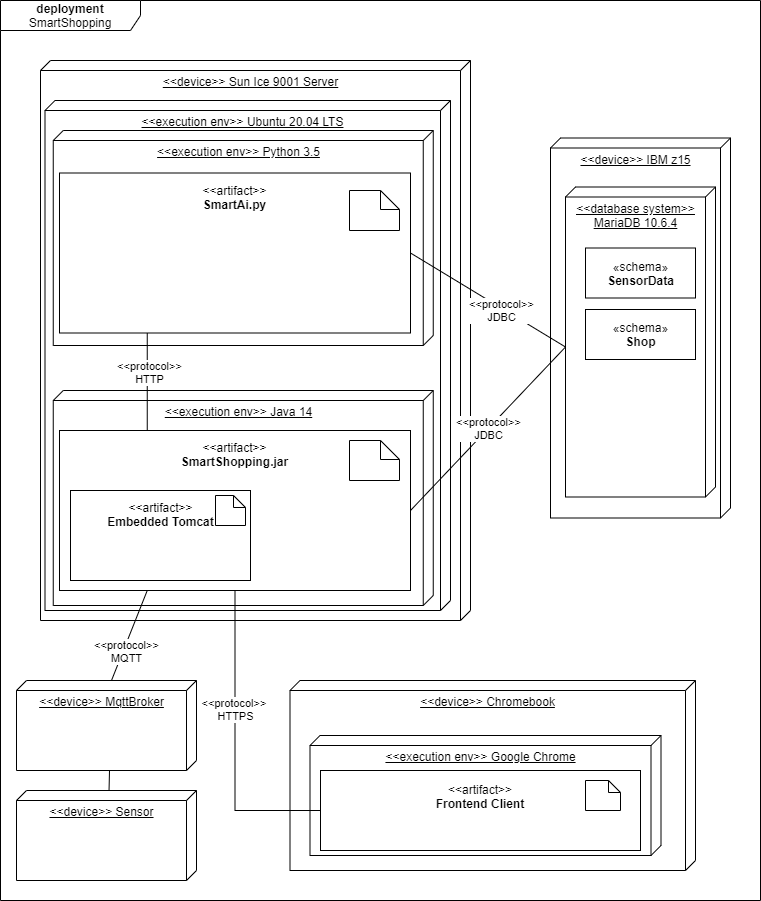
\includegraphics[width=\linewidth]{images/deployment_diagram}


\subsection{Beschreibung der Systemarchitektur}


Der Server auf dem die Anwendung läuft ist ein Sun Ice 9001 Server.
Dieser wird mit dem Betriebssystem Ubuntu 20.04 LTS betrieben.
Darin wird zum einen die SmartAi.py ausgeführt, welche in der Laufzeitumgebung(runtime environment) Python 3.5 läuft.
Zum anderen wird dort die SmartShopping.jar in der Laufzeitumgebung Java 14 ausgeführt.
SmartShopping.jar stellt einen Embedded Tomcat bereit.
Die beiden Anwendungen kommunizieren intern via Rest-Schnittellen mit dem HTTP Protokoll.
Mit dem Datenbankserver kommunizieren sie mit dem JDBC Protokoll.
Der Datenbankserver ist ein IBM z15.
Auf diesem läuft ein MariaDB 10.6.4.
Dieser hat die Schemas SensorData und Shop.
Des Weiteren liefert das Backend den Frontend Client aus.
Welcher beispielsweise auf einem Chromebook ausgeliefert werden kann.
Das Frontend kann dann zum Beispiel in Google Chrome aufgerufen werden.
Backend und Frontend kommunizieren mit dem HTTPS Protokoll.
Außerdem wird im Verteilungsdiagramm ein MqttBroker und die dazu gehörenden Sensoren dargestellt.
Da der Fokus nicht auf dem erheben der Daten liegt, wird nicht näher auf den MqttBroker und die dazu gehörenden Sensoren eingegangen.

\subsection{Einordnung der Architekturentscheidungen}
Der Architekturstil nach Starke ist ein Heterogenes System, da die Kommunikation zwischen den Services über Rest Schnittstellen realisiert ist.
Des Weiteren erfolgt die Kommunikation zwischen Anwendung via HTTP, HTTPS und JDBC.
Die Architektur wurde gewählt, um die Anwendung möglichst modular zu halten und so eine gute Austauschbarkeit von Komponenten zu gewährleisten.

\newpage
\section{Entwurfsmuster}

\subsection{Darstellung der Entwurfsmuster als Klassendiagramm}
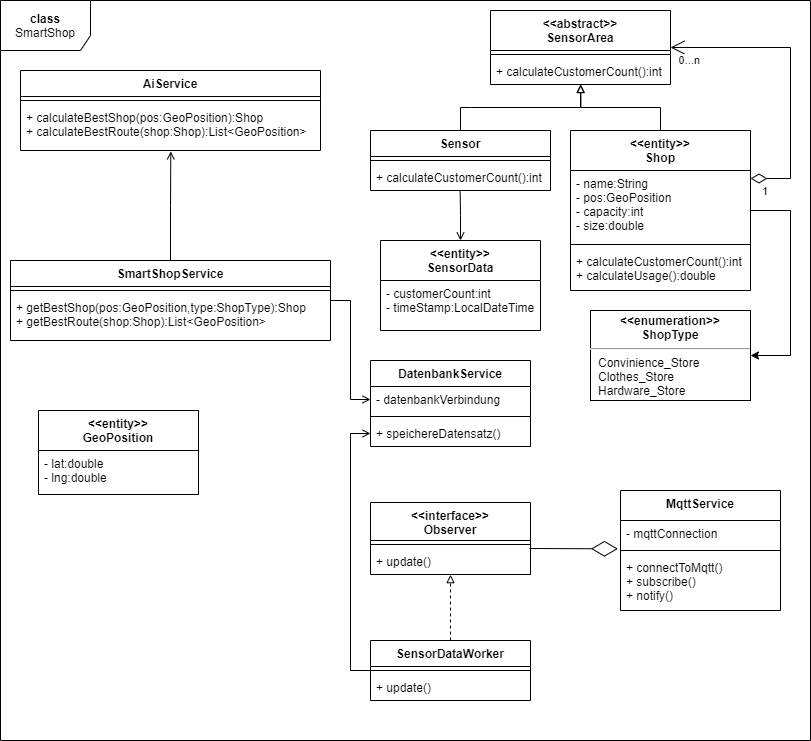
\includegraphics[width=\linewidth]{images/OOD-Klassendiagram}
\begin{description}
\item[Komposit]
Das Komposit ist so umgesetzt, sodass Komplexe Strukturen wie zum Beispiel Einkaufszentren dargestellt werden können.
Dafür wird die abstrakte Klasse SensorBereich (SensorArea) genutzt. Diese besitzt die Methode zur Berechnung der Auslastung, dazu muss jeweils die Auslastung der darunter liegenden Läden(Shop) ebenfalls berechnet werden.
Ein Laden besteht dabei aus mindestens einem Sensorbereich, wobei dieser aus weiteren Läden besteht oder aus konkreten Sensoren(Sensor).
Dadurch kann der Sensorbereich beliebig skaliert und die eigentliche Auslastung rekursiv berechnet werden.  
Diese Skalierbarkeit ist der Vorteil dieses Entwurfsmusters und wurde deswegen ausgewählt. 
\item[Beobachter-Muster]
Für das Beobachter-Muster wurde zunächst die Klasse MqttService modelliert. 
Dieser nimmt Sensordaten vom Mqtt-Sensordaten-Server entgegen.
Damit diese Daten in das richtige Schema der Datenbank persistiert werden können, bietet der Service die Möglichkeit sich darauf einzutragen (subscribe).
Eingetragene Beobachter (Observer) werden über eingehende Sensordaten informiert.
Für die Beobachter wird eine Schnittstelle (Interface) bereit gestellt.
Diese Schnittstelle wird von einer konkreten Klasse implementiert, dem SensorDataWorker.
Dieser SensorDataWorker filtert die Daten, ruft den DatenbankService auf und übergibt die relevanten Daten.
Durch dieses Beobachter-Muster ist es möglich weitere Daten über separate Beobachter zu verarbeiten, ohne das bisherige Beobachter angepasst werden müssen.
\end{description}


\subsection{Begründung}
Der Vorteil des Kompositum-Musters ist, dass der Sensorenbereich (SensorArea) beliebig erweitert werden kann und es dabei zweitrangig ist um was die Shops beziehungsweise andere Komponenten erweitert werden. 
Ein Nachteil dabei ist, dass die Tiefe ebenfalls beliebig wächst und es so zu einer sehr unübersichtlichen Datenstruktur kommen kann.
Eine Alternative beziehungsweise Erweiterung wäre das Fabrikmethode-Muster. 
Dieses Muster erlaubt es uns auf Grundlage der abstrakten Klasse SensorArea weitere Bereiche zu implementieren, ohne dass davon andere Services betroffen sind. 
Man könnte also Shop oder Einkaufszentrum erzeugen, würde dabei aber die Möglichkeit der Schachtelung verlieren. 
Um beide Entwurfsmuster möglichst effektiv zu verwenden, wäre eine Kombination denkbar.
\\


Das Beobachter-Muster wurde gewählt, da es eingehende Signale von den Sensoren beziehungsweise Sensornachrichten automatisch verarbeitet und speichert.
Dieses Muster könnte durch das Zustands-Muster erweitert, aber nicht ersetzt werden.
Das Zustands-Muster würde in der konkreten Implementierung ebenfalls auf eingehende Nachrichten warten / reagieren, es könnte beispielsweise als ein Buffer agieren welcher Nachrichten sammelt und erst auf Anfrage Daten weiter leitet / speichert.
Dieses Verhalten würde das Beobachter-Muster eher erweitern oder imitieren und ist daher ungeeignet in diesem Kontext.


\newpage
\section{Beschreibung der Kernfunktionalität}
Eine der Kernfunktionalitäten ist es, die Auslastung von Shops zu ermitteln und mit dieser Information weiter zu arbeiten.
Daher stellen wir in diesem Abschnitt die Funktionalität zur Ermittlung der Auslastung eines Einkaufzentrums (ShoppingCenter) dar.

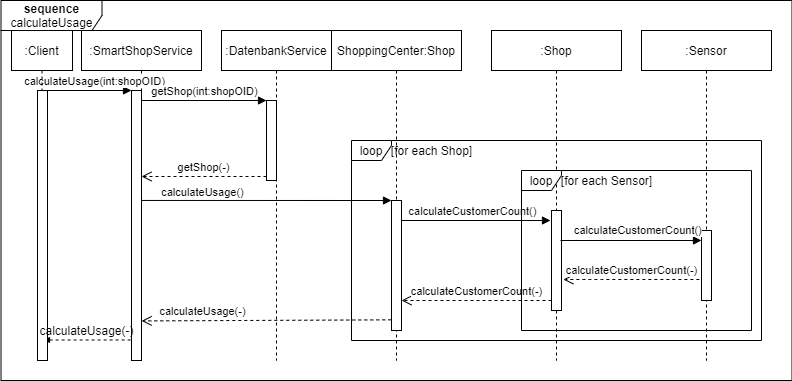
\includegraphics[width=\linewidth]{images/Sequenzdiagramm}
In dem Sequenzdiagramm beschriebenen Beispiel, möchte ein Client die Auslastung eines bestimmten Shops haben und ruft daher die Methode calculateUsage auf dem SmartShopService auf.
\\

\textbf{SmartShopService}: In diesem Beispiel wird davon ausgegangen, dass es bei der Auflösung einer bestimmten ShopOID nicht zu einem Fehler kommt sondern die Auflösung immer erfolgreich ist.
Die Methode \textbf{\textit{calculateUsage}} berechnet die aktuelle Auslastung des Shops welcher über seine ShopOID angefordert wird.
\begin{lstlisting}[language=Java, basicstyle=\scriptsize]
public int calculateUsage(int shopOID){
	Shop tmp = datenbankService.getShop(shopOID);
	return tmp.calculateUsage();
}
\end{lstlisting}


\textbf{DatenbankService}: Beim Aufruf der Datenbank wird davon ausgegangen, dass es zu keinem Fehler kommt und die Datenbank den Shop mittels Primärschlüssel findet.
Die genaue Anfrage an die Datenbank wird durch die Funktion \textbf{\textit{getShopByPrimaryKey}} abstrahiert.
\begin{lstlisting}[language=Java, basicstyle=\scriptsize]
public Shop getShop(int shopOID){
	return getShopByPrimaryKey(shopOID);
}
\end{lstlisting}

\break
\textbf{Shop}: Die Methode \textbf{\textit{calculateCustomerCount}} iteriert über die Liste seiner Sensoren und summiert deren Kunden auf.
Darauf hin iteriert die Methode über die Shops die dem aktuellen Shop zugeordnet sind und ruft darauf \textbf{\textit{calculateCustomerCount}} auf, um die Anzahl der zurück gegebenen Kunden aufzusummieren.
Die Methode liefert die aufsummierte Anzahl an Kunden pro Shop und Sensor zurück.
\begin{lstlisting}[language=Java, basicstyle=\scriptsize]
public int calculateCustomerCount(){
	int customerCount = 0;
	List[Shop] shopList;
	List[Sensor] sensorList;
	for(Sensor sensor : sensorList){
		customerCount += sensor.getCustomerCount();
	}
	for(Shop shop : shopList){
		customerCount += shop.calculateCustomerCount();
	}
	return customerCount;
}
\end{lstlisting}

Die Methode \textbf{\textit{calculateUsage}}, berechnet die momentane Auslastung eines Shops, basierend auf seiner Kapazität, der aktuellen Anzahl seiner Kunden und der Anzahl von Kunden seiner Shops.
\begin{lstlisting}[language=Java, basicstyle=\scriptsize]
public int calculateUsage(){
	int customerCount = 0;
	List[Shop] shopList;
	List[Sensor] sensorList;
	for(Shop shop : shopList){
		customerCount = shop.calculateCustomerCount();
	}
	for(Sensor sensor : sensorList){
		customerCount = sensor.getCustomerCount();
	}
	return capacity - customerCount;
}
\end{lstlisting}

\newpage
\section{Persistente Datenhaltung}

\subsection{Persistierungansatz}
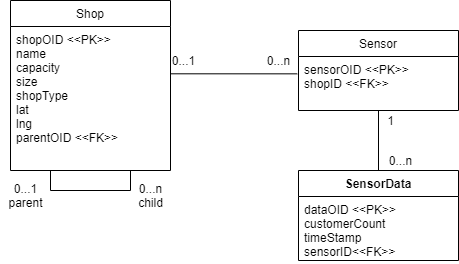
\includegraphics[width=\linewidth]{images/Datamodel}
\begin{description}
	\item[Shop] Der Shop besitzt eine eindeutige ID, welche als Primärschlüssel dient. 
	Des weiteren die Felder: 
	\begin{description}
		\item [name:] Das Feld name repräsentiert den Namen des Shops.
		\item [capacity:] Für die maximale Anzahl an Kunden im Shop.
		\item [size:] Das Attribut size beschreibt die Grundfläche des Shops.
		\item [shopType:] ShopType repräsentiert den Typen des Shops.
		\item [lat, lng:] lat, lng beschreiben den Breitengrad, Längengrad des Shops. Breitengrad und Längengrad kommen aus der Entität \textbf{GeoPosition}, welche aber in diesem Kontext in Shop persistiert werden, da sie in einer eins zu eins Beziehung stehen.
		\item [parentOID:] Repräsentiert einen Fremdschlüssel auf einen möglicherweise übergeordneten Shop, das Feld kann leer sein.
	\end{description} 
	Die Parent-Child-Beziehung beschreibt, das im Entwurfsmuster dargestellte Komposit.
	\item[Sensor] Der Sensor besitzt das Feld sensorOID, welches eine eindeutige ID ist und als Primärschlüssel fungiert. Außerdem besitzt es das Feld shopOID als Fremdschlüssel, welcher auf einen eindeutigen Shop zeigt, das Feld kann leer sein.
	\item[SensorData] SensorData besitzt die Felder:
	\begin{description}
		\item[dataOID:] Die dataOID fungiert als ID und einzigartiger Primärschlüssel.
		\item[customerCount:] Das Feld customerCount repräsentiert die Anzahl an Kunden zu dem Zeitpunkt des Erstellens von SensorData.
		\item[timeStamp:] Dieses Feld enthält den Zeitpunkt zu dem SensorData erstellt wurde.
		\item[sensorOID] SensorOID enthält einen Fremdschlüssel, welcher den zu SensorData gehörenden Sensor identifiziert.
	\end{description}
\end{description}

In der Datenhaltung werden die Entitäten Shop, Sensor und Sensordaten (SensorData) gespeichert.
Eine weitere Entität wäre die geografische Position, da diese aber in einer eins zu eins Beziehung zur Entität Shop steht, werden die Daten direkt in Shop integriert.

Der DatenbankService verwendet JPA und setzt dabei auf einen Entity Manager.
Die gewählte Datenbank ist eine MariaDB, welche auf einem eigenen Server ausgeliefert wird.


\subsection{Begründung}
Da die Daten einfach strukturiert sind und eine eindeutige ID besitzen, habe ich mich für eine SQL Datenbank entschieden.
Durch diese Datenstruktur ist ein schneller, sicherer und einfacher Zugriff möglich.
Die gewählte Datenbank ist eine MariaDB, da diese frei verfügbar ist (OpenSource) und von Michael Widenius, dem Entwickler von MySQL, entwickelt wurde.
Die Datenbank wird auf einem eigens dafür vorgesehenen Server aufgesetzt, um eine lose Kopplung zu gewährleisten. Außerdem können Anwendungen, anders als bei einer In-Memory Datenbank, unabhängig voneinander auf die Datenbank zugreifen.
Ich habe mich für JPA entschieden, da es durch Spring standardisiert ist und datenbankunabhängig funktioniert. Der Nachteil an JPA ist, dass weitere Abhängigkeiten in den Code geladen werden.

Eine Alternative zu MariaDB wäre eine NoSQL Datenbank, ich habe mich dagegen entschieden, da ich mit einem festen Schema arbeiten möchte und NoSQL das nicht bietet.
Für eine NoSQL Datenbank würde sprechen, dass man die Sensordaten welche mit einem Zeitstempel versehen werden in eine Zeitreihen-Datenbank auslagern kann.

Weitere Datenbankenmodelle wären zum Beispiel eine dokumentenorientierte Datenbank oder Graphdatenbank. Beide Modelle eignen sich für diesen Anwendungsfall nicht, da weder mit Dokumenten noch mit Graphen gearbeitet wird.
\newpage

\section{Kommunikation}

\subsection{Kommunikationsansatz}
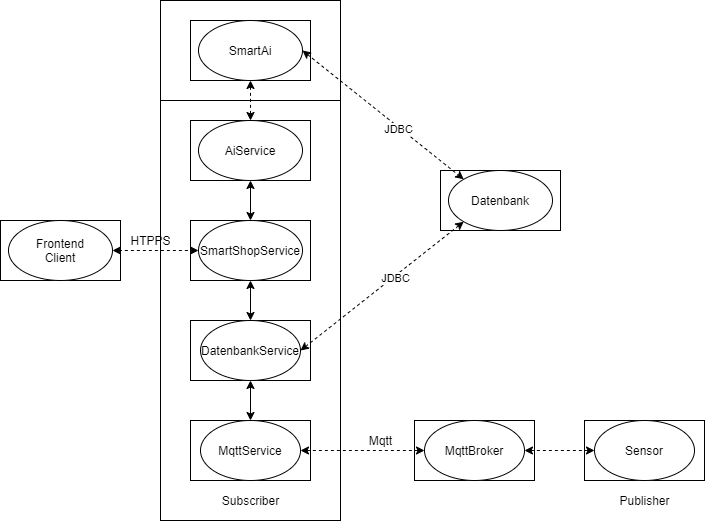
\includegraphics[width=\linewidth]{images/Kommunikation}

Die Kommunikation zwischen SmartAI und dem AiService erfolgt über REST-Schnittstellen mit dem HTTP-Protokoll, diese Kommunikation ist synchron.

Die SmartAi kommuniziert mit dem Datenbankserver via JDBC, diese Kommunikation ist ebenfalls synchron. JDBC ist eine Middleware, welche ein standartisiertes Interface für SQL Datenbanken bereit stellt.

Der Frontend Client kommuniziert mit dem SmartShopService mit HTTPS über eine REST-Schnittstelle. Die Kommunikation ist synchron.

Der DatenbankService kommuniziert ähnlich wie die SmartAi über JDBC mit der Datenbank. Die Kommunikation ist synchron und JDBC ist eine Middleware.

Der MqttService funktioniert nach dem Publish-Subscribe Prinzip. Der MqttService abonniert (subscribed) die Nachrichten vom MqttBroker, welcher wiederum die Nachrichten der Sensoren sammelt und an seine Abonnenten (Subscriber) weiter leitet.
Der MqttBroker dient als Middleware, es wird das MQTT-Protokoll verwendet und die Kommunikation ist asynchron. \\

Die nach außen bereitgestellten Schnittstellen sind vom Backend ausgehend REST-Schnittstellen, um Metainformationen anzufordern, wie zum Beispiel die aktuelle Auslastung eines Shops.
Außerdem eine Schnittstelle die den besten Weg basierend auf beispielsweise dem aktuellen Standort, der bei der Anfrage mit geliefert wird, zurück gibt.
Diese Schnittstellen werden im Regelfall vom Frontend angesprochen.

Außerdem stellt der Datenbankserver eine Schnittstelle bereit, um mit SQL Daten anzufordern/zu speichern, allerdings wird diese nur vom Backend angesprochen und sollte von außen nur gesichert erreichbar sein. \\

\subsection{Begründung}
Die REST API wird in diesem Kontext verwendet, da sie eine einfache und standardisierte Kommunikation zwischen Services in einem verteilten System darstellt.
Dadurch ist gewährleistet, dass weitere Services einfach erweitert, ergänzt und ersetzt werden können, ohne die Schnittstelle selbst zu verändern.

Eine Alternative wäre es, Services direkt über die jeweilige IP anzusprechen.
Der Vorteil wäre, dass man dadurch eine größere Flexibilität und eine bessere Performance realisieren kann.
Der Nachteil dabei ist, dass der Programmierer die Kommunikation selbst implementieren muss und anpassen muss, sollte es zu Änderungen im System kommen.
Außerdem bietet REST die Möglichkeit Services einfach nach außen, beispielsweise ins World Wide Web, verfügbar zu machen.

JDBC wird verwendet, da die Middleware ein standardisiertes Interface bietet und somit der Programmierer einfach mit dem Datenbank Server kommunizieren kann.
Ähnlich wie bei REST könnte man auch hier eine direkte Kommunikation implementieren, muss dann allerdings auch den Aufwand betreiben und bei Änderungen die Kommunikation anpassen.

Der MqttBroker wird in diesem Kontext verwendet, da er die Kommunikation mit den Sensoren vereinfacht.
So muss der Programmierer sich nicht darum kümmern wie viele Sensoren existieren und muss nur eingehende Änderungen verarbeiten.
Hier wieder das Problem, man muss über eine Middleware arbeiten, welche nicht zwangsläufig optimiert funktioniert.


\newpage
\bibliography{lit}
Tilkov, Stefan, et al. REST und HTTP: Entwicklung und 
Integration nach dem Architekturstildes Web. dpunkt. verlag, 
2015
\bibliographystyle{alpha}

\end{document}
